\documentclass{article}

\usepackage{physics}
\usepackage{amsmath, amsfonts, amsthm}
\usepackage{graphicx}
\usepackage{float}

\begin{document}

\section{Intro} % (fold)
\label{sec:Intro}

\begin{align}
    \qty(1+\epsilon)^r&=\sum_{n=0}^\infty
    {r\choose2}\epsilon^n\\
                      &=\sum_{n=0}^\infty C_r\epsilon^n
\end{align}

Ceci est la formule du binôme de Newton.\\
Elle est très utile.

\begin{align}
    &\vb{v}=\dv{\vb{r}}{t}=\dot{\vb{r}} &&\vb{a}=\dv{\vb{v}}{t}=\ddot{\vb{r}}\\
    &\vb{v}=\frac{d\vb{r}}{dt}
\end{align}

Maintenant, les matrices.

\begin{align}
    \sigma_x&=\mqty(0 & 1 \\ 1 & 0)\\
    \sigma_y&=\mqty[0 & -i \\ i & 0]
\end{align}

\begin{figure}[H]
    \begin{center}
        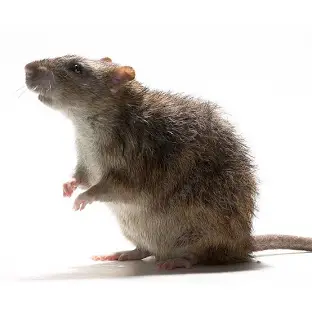
\includegraphics[width=0.95\textwidth]{rat.png}
    \end{center}
    \caption{Il n'y a pas de rats en Alberta}\label{fig:}
\end{figure}
Notes pour nabla,

\begin{align}
    f(x) & =xy^2\\
    \nabla f&=\mqty(y^2\\2xy)\\
    \boldsymbol{\nabla}\cdot\nabla f&=2x
\end{align}

\begin{align}
    \int_{-\infty}^\infty e^{-x^2/2\sigma^2}\dd{x}&=\sqrt{2\pi}\sigma
\end{align}

% section Intro (end)

\section{Figure}

\begin{align}
    \int\dd{\int}
\end{align}



\end{document}
